%!TEX root = ..//Avali-Arena-Esportivas.tex
\section{MÉTODO EVOLUTIVO}
\subsection{DETERMINAÇÃO DO VALOR TOTAL DA ARENA}
\begin{equation}
	Metodologia - Valor \, Total \, do \, Imovel - Metodo \, Evolutivo
\end{equation}

%
\hspace*{1.25 cm} Em função das características do imóvel avaliando, do mercado imobiliário local e da pesquisa realizada adotou-se o método acima por ser o que melhor reflete a realidade do imóvel avaliando.\\ 
%
\hspace*{1.25 cm} Diz a Norma: “\textit{8.2.4 - A composição do valor total do imóvel avaliando pode ser obtida através da conjugação de métodos, a partir do valor do terreno, considerados o custo de reprodução das benfeitorias devidamente depreciado e o fator de comercialização}”, ou seja:\\

\begin{minipage}[t!]{0.35\textwidth}
	\begin{equation}
		VI = (VT + CB) x FC  
	\end{equation}		
	
\end{minipage}\hfill
\begin{minipage}[t!]{0.5\textwidth}
	Onde:\\ 
	VI =	Valor do imóvel\\ 
	VT =	Valor do terreno\\ 
	CB =	Custo de reedição da benfeitoria\\ 
	FC =	Fator de comercialização\\ 
\end{minipage} 


\begin{figure}[H]
	\centering  \small 		\caption{ Amostra do Tratamento Estatístico do terreno}
	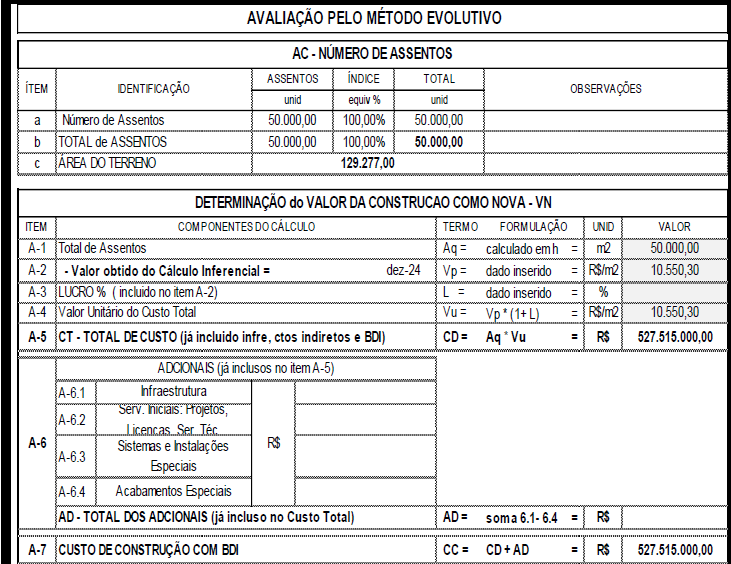
\includegraphics[width=0.94947\linewidth]{figura/screenshot039}
	\label{fig:screenshot039}\\{ Fonte: Elaborado pelos Autores }
\end{figure}

\begin{figure}[H]
	\centering  \small 		\caption{ Amostra do Tratamento Estatístico do terreno}
	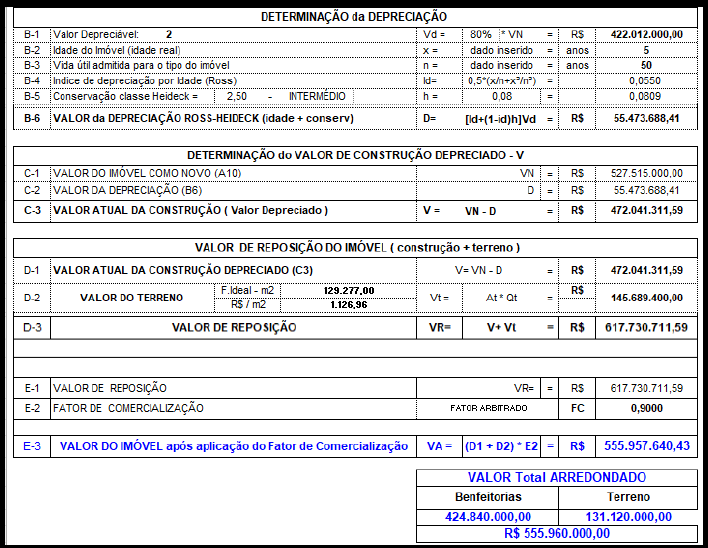
\includegraphics[width=0.94947\linewidth]{figura/screenshot040}
	\label{fig:screenshot040}\\{ Fonte: Elaborado pelos Autores }
\end{figure}

\begin{comment}
	AVALIAÇÃO PELO MÉTODO EVOLUTIVO					\\ 
	AC - NÚMERO DE ASSBNTOS					\\ 
	ÍTEM	IDENTIFICAÇÃO	ASSENTOS	INDICE	TOTAL	OBSERVAÇÕES\\ 
	unid	equiv \%	unid	\\ 
	Número de Assentos	50.000,00	100,00\%	50.000,00 :	\\ 
	TOTAL de ASSENTOS	50.000,00	100,00\%	50.000,00 ?	\\ 
	ÁREA DOTÍR'RBNO'	129.277,00 í			\\ 
	DETERMINAÇÃO do VALOR DA CONSTRUCAO COMO NOVA - VN\\ 
	ITEM	COMPONENTES DO CÁLCULO				TERMO FORMULAÇÃO	UNID	VALOR\\ 
	A-1	Total				Aq = calculado emh =	m2	50.000,00\\ 
	A-2	-Valor obtido do Cálculo Inferencial = dez-24				Vp = dado inserido =	R\$/m2	10.550,30\\ 
	A-3	LUCRO \% (incluido no item A-2)				L = dado inserido =	\%	\\ 
	A-4	Valor Unitário do Custo Total				Vu = Vp * (1 + L) =	R\$/m2	10.550,30\\ 
	A-5	CT - TOTAL DE CUSTO (já incluido infre, ctos indiretos e BDI)				CD= Aq*Vu =	R\$	527.515.000,00\\ 
	A-6	ADCICNAIS (já inclusos no item A-5)						\\ 
	A-6.1	Infraestrutura	R\$				\\ 
	A-6.2	''Serv. Iniciais:'Projetos,''					\\ 
	A-6.3	Sistemas e Instalações Especiais					\\ 
	A-6.4	Acabamentos Especiais					\\ 
	::-¦:¦:.:::::: :V : : ¦				AD = soma6.1-6.4 = f R\$		\\ 
	%A-7	CUSTO DE CONSTRUÇÃO COM BDI				CC =	cD + AD	= |'R\$			527.515.000,00\\ 
	Fonte - elaborado pelos autores\\ 
	Fonte - elaborado pelos autores\\ 
	
\end{comment}